\chapter{Theory}
This chapter contains the necessary theory for SRON-GAN. A brief introduction to exoplanets and their formation is made, with a follow up of atmospheric retrieval. After which a brief introduction to neural networks is given and two types of GANs with their use for semantic image inpainting are presented. Finally, recent developments are discussed and ExoGAN is presented.

%%%%%%%%%%%%%%%%%%%%%%%%%%%%%%%%%%%%%%%%%%%%%%%%%%%%%%%%%%%%%%%%%%%%%%%%%%%%%%%%%%
\section{Exoplanets}
The journey from cosmic dust to grain growth and eventually the formation of planetesimals or exoplanets is a subject which is currently actively being studied. Figure \ref{fig:protodisk} shows a visualisation of a protoplanetary disk \cite{henning2013chemistry}. Going from left to right, cosmic dust with a initial size of about a $\mu$m has a chance to collide with one another after which it sticks together due to the Van der Waals force, enlarging the grain size over time to about a mm. After this process the dust start to settle down to the mid-plane of the protoplanetary disk, increasing to about a meter in size. Finally gravity starts to have an important role, where objects of about one km in size are created. 

Overtime planets of about one M$_{\bigoplus}$ have a chance to be created, where M$_{\bigoplus}$ is the Earth mass. At this point the planet could start to form an atmosphere by attracting material from the protoplanetary disk. There are lots of possibilities for the types of planets to be formed, resulting in planetary systems completely different from the Solar System. This research focuses on Hot Jupiters. Hot Jupiters are gas giants, which are expected to initially start out with a planet size of about 10 M$_{\bigoplus}$. Their relatively large mass allows for the aggregation of lots of material. While the planet orbits the star, it essentially aggregates most of the material it passes through. After which the planet slowly spirals to an orbit close to the star.

The right part of Figure \ref{fig:protodisk} visualises at which point in the protoplanetary disk, which processes take place. Relevant to the formation process is e.g. where within the disk the planet has formed. This determines the physical and chemical processes taking place, having an influence on the internal temperature, the accretion of solids and water ice within the atmosphere, and the other features as discussed in Chapter \ref{atm_retrieval}. Most of this information is encoded into the footprint of the respective exoplanet, its atmospheric composition.




\begin{figure} [!htb]
    \centering
    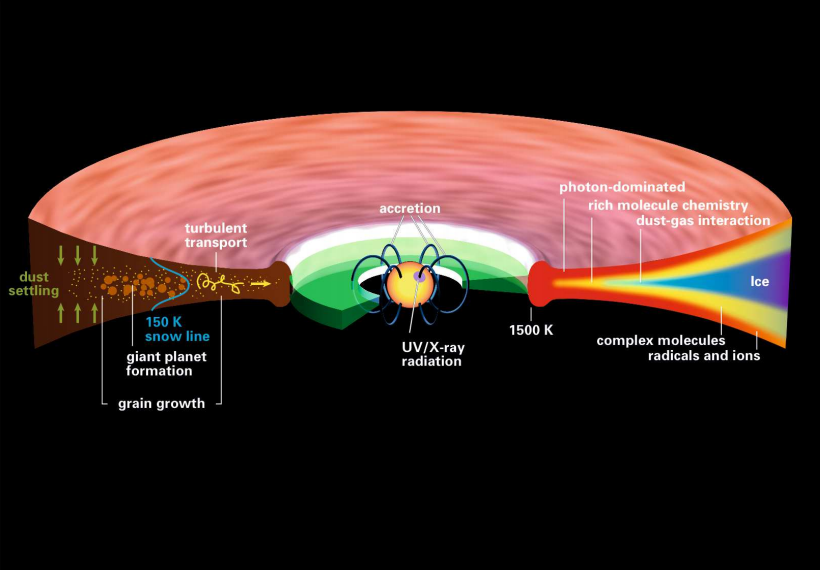
\includegraphics[scale=0.5]{figuren/protodisk.png}
    \caption{Sketch of the physical and chemical structure of a protoplanetary disk around a Sun-like star\cite{henning2013chemistry}. Figure source: \cite{henning2013chemistry}}.
    \label{fig:protodisk}
\end{figure}


\subsection{Atmospheric Retrieval and Forward Modelling} \label{atm_retrieval}
To get a better understanding of the forming scenarios and evolution of exoplanets, it is required to comprehend their atmospheric compositions. To do this, physically complex retrieval models are required. These retrieval codes consist of a forward model and an inference method. Whereas the forward model creates an atmospheric spectrum, given the model parameters. The inference method takes an atmospheric spectrum and returns the corresponding model parameters with their uncertainties.

The forward model computes the transmission and transmission spectra, given the input parameters. Such input parameters are e.g. the planet radius, planet mass, planet temperature and the carbon to oxygen ratio. The process of forward modelling is summarised in the following way. The forward model computes the atmospheric structure and opacity, performs radiative transfer and repeats this process until a chemical and physical equilibrium has been reached, i.e. the model has converged. After which a model spectrum is returned. The aim of the inference method is to fit an atmospheric model to the observed spectrum and return the model parameters with their uncertainties. The observed spectrum along with its uncertainties is given as an input, upon which an inference method of choice is used to retrieve the corresponding atmospheric model. Bayesian inferences methods like Markov Chain Monte Carlo (MCMC) and Nested Sampling (NS) are most commonly used for this process \cite{madhusudhan2018atmospheric}. 

There are lots of exoplanetary atmospheric retrieval codes \cite{madhusudhan2009temperature, line2013systematic, irwin2008nemesis, benneke2012atmospheric, waldmann2015tau, lavie2017helios, gandhi2017retrieval}. Some of these use less common inference methods like a grid search, while others use MCMC, NS, Optimal Estimation (OE) and Bootstrap Monte Carlo (BMC) \cite{line2013systematic}. The same goes for the varying complexity in the use of physical and chemical models. Certain retrieval codes solely use a simplistic physical model, utterly leaving out any chemistry or more complex and realistic physics. While other retrieval codes go to the other extreme, with complex physical models and (non-)equilibrium chemistry. Both sides come with their own consequences. The former returns a rough estimate of the atmospheric model, requiring little computational power. While the latter returns an atmospheric model that corresponds more to reality, requiring lots of computational power. The retrieval with a simple model could take about ten CPU core hours until convergence, while a complex model requires thousands of CPU core hours \cite{zingales2018exogan, madhusudhan2018atmospheric}.

One example of an exoplanetary retrieval code which uses physically complex models is the ARCiS framework for exoplanet atmospheres \cite{min2019arcis}. ARCiS is currently being developed by Michiel Min at SRON. It includes anisotropic scattering, molecular chemistry, a self consistent temperature-pressure profile and cloud formation \cite{ormel2019arcis}. The capacities of molecules are calculated by using the ExoMol line lists and correlated k-tables \cite{tennyson2016exomol, ormel2019arcis}. The aim of ARCiS is to use the parameters of the planet formation process and its evolution, to be able to predict observable quantities within the transmission and transmission spectra \cite{min2019arcis}. To create a forward model, ARCiS takes the planet parameters and processes them as visualised in Figure \ref{fig:arcis_schem}. The final output is the best corresponding atmospheric model, including its features. Both the parameters and features are listed in Table \ref{table:srongandatasetparameters}. In machine learning jargon it's common to call anything which is predicted a feature. Since SRON-GAN will predict both the parameters and features, both are referred to as features within the SRON-GAN concept.

\begin{figure} [!htb]
    \centering
    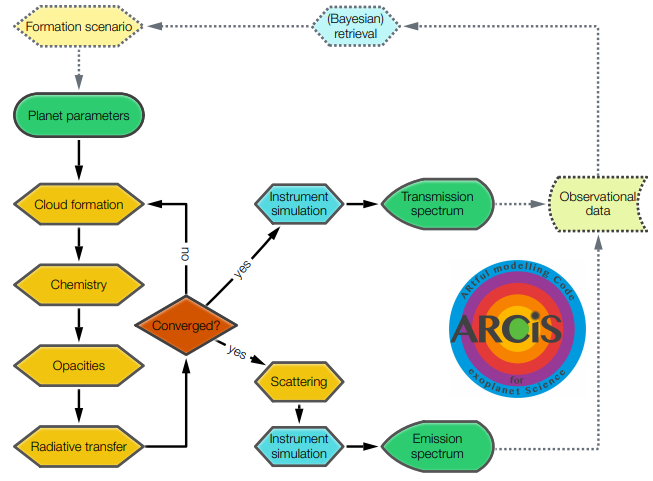
\includegraphics[scale=0.6]{figuren/ARCiS_schematic.png}
    \caption{A schematic representation of the modelling chain from the ARCiS framework. Figure source: \cite{min2019arcis}}.
    \label{fig:arcis_schem}
\end{figure}

\begin{table}[!htb]
\caption{The atmospheric model parameters. Where $\mathrm{R_J}$ and $\mathrm{M_J}$ are the Jupiter radius and Jupiter mass respectively. The abundances parameter refers to the abundances of $\mathrm{CH_4 , CO_2 , CO , H_2O , C_2H_2 , C_2H_4 , H_2 , HCN , He , K , NH_3 , Na , SO_2 , TiO}$ and VO. The formation temperature has a fixed value of 100 K and the host stars radius R$_*$ has a fixed value of 1 Solar radius, R$_\odot$.}
\label{table:srongandatasetparameters}
\resizebox{\columnwidth}{!}{%
\begin{tabular}{|c|l|c|c|}
\hline
\textbf{Feature} & \multicolumn{1}{c|}{\textbf{Description}}                                                                                            & \textbf{Sampling method}                                                            & \textbf{Unit} \\ \hline
Dplanet          & Distrance between the planet and host star.                                                                                           & $\log_{10}$                                                                               & AU                 \\ \hline
Rp               & Planet radius                                                                                                                        & linear                                                                              & $R_J$               \\ \hline
Mp               & Planet mass                                                                                                                          & linear                                                                              & $M_J$               \\ \hline
betaT            & Efficiency of incoming radiaton.                                                                                                      & $\log_{10}$                                                                               & -                   \\ \hline
TeffP            & Internal temperature                                                                                                                 & $\log_{10}$                                                                               & K                  \\ \hline
fdry, f\_dry     & Accretion of solid material within the atmosphere.                                                                                    & $\log_{10}$                                                                               & -                   \\ \hline
fwet, f\_wet     & Accretion of water ice within the atmosphere.                                                                                         & $\log_{10}$                                                                               & -                   \\ \hline
cloud1:Sigmadot  & Nucleation speed for the clouds.                                                                                                      & $\log_{10}$                                                                               & g cm^{-2}s^{-1}                   \\ \hline
cloud1:Kzz       & Mixing efficiency for the clouds.                                                                                                     & $\log_{10}$                                                                               & cm^2 s^{-1}                   \\ \hline

COratio          & Ratio between C and O within the atmosphere.                                                                                          & \begin{tabular}[l]{@{}c@{}}Derived from f\_dry and f\_wet in\\   ARCiS\end{tabular} & -                   \\ \hline
metallicity      & Fraction of heavy elements within the atmosphere.                                                                                     & \begin{tabular}[l]{@{}c@{}}Derived from f\_dry and f\_wet in\\   ARCiS\end{tabular} & -                   \\ \hline
T                & \begin{tabular}[c]{@{}l@{}}Temperature at the height of the atmosphere which which contributes most\\   to the spectrum.\end{tabular} & Derived in ARCiS                                                                    & K                   \\ \hline
P                & Pressure at the height from T.                                                                                                        & Derived in ARCiS                                                                    & bar                   \\ \hline
Abuncances       & \multicolumn{1}{l|}{Abundances of the molecules at the height from T.}                                                                & $\log_{10}$                                                                               & -                   \\ \hline
\end{tabular}%
}
\end{table}







%%%%%%%%%%%%%%%%%%%%%%%%%%%%%%%%%%%%%%%%%%%%%%%%%%%%%%%%%%%%%%%%%%%%%%%%%%%%%%%%%%
\section{Neural Networks} \label{neuralnetworks}
Deep learning is a sub-field of machine learning, where algorithms learn to perform a task in a supervised, semi-supervised or unsupervised way, without being explicitly programmed to do so. These algorithms are called artificial neural networks and their design is inspired by how biological neural networks within animal brains work. Lets first take a look at the concepts from a simple neural network, before discussing the Deep Convolutional Generative Adversarial Network (DCGAN) in the next subchapter. The most basic neural network architecture is visualised in Figure \ref{fig:simplednn}. Which translates to the function:
\begin{equation}
    y=f(x_0)=\theta_0 x_0+b_0
\end{equation}

\begin{figure} [!htb]
    \centering
    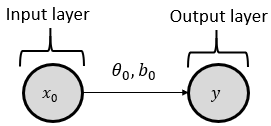
\includegraphics[scale=0.6]{figuren/fig2.2.1.1.png}
    \caption{A schematic representation of the most basic neural network architecture, consisting of one input node and one output node, without any hidden layers inbetween.}
    \label{fig:simplednn}
\end{figure}

Where $x_0$ is the model input, $\theta_0$ is the weight from the input neuron to the output neuron and $b_0$ is the bias, also known as offset. In general $\theta_0$ and $b_0$ are called the weights of the model. This model could be used to learn any linear relationship between two variables. This is done is by randomly initialising the weights at the start of training. The first input value goes into the model and the models prediction $y$ is calculated, this is called a forward pass. After which the loss, resulting from the loss function, between the prediction $y$ and ground truth value $\hat{y}$ is calculated. In a regression problem the loss function could be e.g. the mean squared error. Once the loss is known, backpropagation is performed to calculate the gradient of the network. After which gradient descent is used to change the weights in such a way that it minimises the value of the loss function. 

In practise this process is not performed on a single input value. Usually  backpropagation is performed after a single batch or a complete epoch. If for example the complete training dataset consists of 512 samples, i.e. 512 input values with their corresponding ground truth values. One epoch would be a forward pass through the complete dataset. In this case the average value of the loss function is, together with the average gradient, followed up by backpropagation. This allows for a more smooth execution of gradient descent. Sometimes it is the case that the complete dataset does not fit into the video or computer memory. This is where batches come into play. A batch is a sample of samples from the dataset. When for example a batch size of 64 is used, backpropagation is performed after 64 samples. Meaning that during one epoch, 8 batches are forward passed and backpropagation with gradient descent is performed 8 times. Of course this is all customizable. Batches could be used despite the dataset fitting into memory, because of performance reasons. Back propagation may also be used after the 8 batches, on the average gradient from those batches. Certain methods are a matter of preference and choice, but might highly influence the training process of a neural network.

The power of neural networks lies into the ability for them to learn non-linear relationships between their input $x$ and output $y$. A simple Deep Neural Network (DNN) which has this ability is made by taking the building blocks from Figure \ref{fig:simplednn} and using them to create an architecture as visualised in Figure \ref{fig:deepdnn}. Where in Figure \ref{fig:simplednn} the weights are linearly forward passed, here each neuron also has an activation function $f_{acc}$. Meaning that the summation of the previously connected neurons is fed into the activation functions, to add non-linearity to the model. One of the most common activation function is called the Leaky Rectified Linear Unit (Leaky ReLU) and is visualised in Figure  \ref{fig:leakyrelu} \cite{xu2015empirical}. It is quickly seen that by configuring these building blocks in different ways, arbitrary complex architectures can be created. But no matter how complex, it all breaks down to the transformation:
\begin{equation}
    f(\boldsymbol{x}) \rightarrow \boldsymbol{y}
    \label{eq:mapping}
\end{equation}
Where $\boldsymbol{x}$ represents the model input, $\boldsymbol{y}$ the model output and the function $f$ is the model itself.

\begin{figure} [!htb]
    \centering
    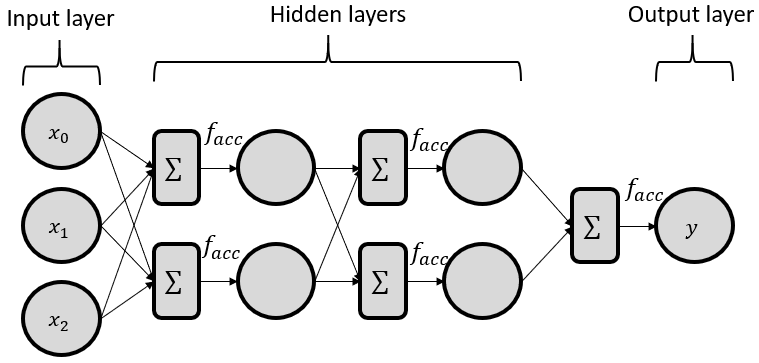
\includegraphics[scale=0.5]{figuren/fig2.2.1.2.png}
    \caption{A schematic representation of a deep neural network, consisting of so called linear layers. The input is a 3 dimensional vector, $\boldsymbol{x}=[x_0, x_1, x_2]$. There are two hidden layers, both consisting of 2 nodes each. Finally, there is one single node at the output layer.}
    \label{fig:deepdnn}
\end{figure}

\begin{figure} [!htb]
    \centering
    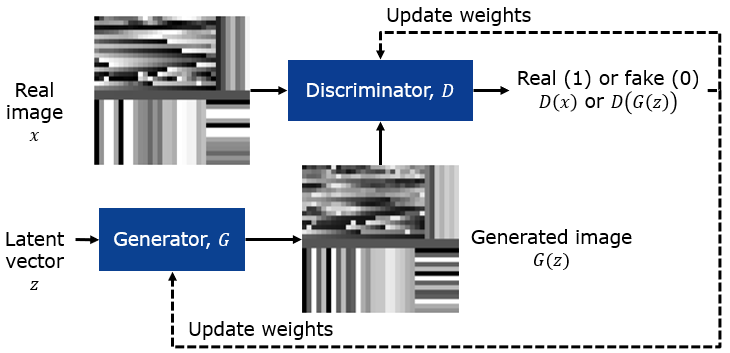
\includegraphics[scale=0.5]{figuren/fig3.png}
    \caption{A schematic representation of GAN training.}
    \label{fig:gantraining}
\end{figure}






\subsection{Deep Convolutional Generative Adversarial Networks}
Most neural networks are designed to purely make a prediction depending on its input data. A model could take an image of a dog as an input and classify the image as a dog. However, this still simply is a mapping of the input image to the model output as described in Equation \ref{eq:mapping}. The model has learned how to recognise a dog, but it cannot be used to e.g. create images of artificially generated dogs. This is where the Generative Adversarial Network (GAN) comes in. The following subchapters presents different rigorous mathematical equations on the loss functions used in these type of models. They are simplified in Subchapter \ref{lossfunctions_subchapter}.

\begin{figure} [!htb]
    \centering
    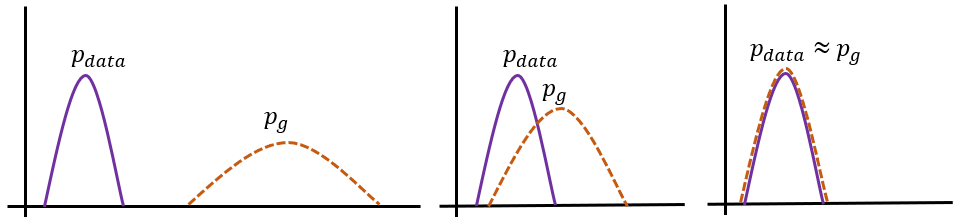
\includegraphics[scale=0.5]{figuren/gan real fake distributions learning.png}
    \caption{The process where the generator from a GAN learns to approximate the real data distribution. Upon training, the generators data distributions changes in such a way that it ideally starts to look like the real data distribution. $\textbf{Left}$: At the start of training the generators data distribution $p_g$ does not match the real data distribution $p_{data}$. $\textbf{Centre}$: Somewhere in the middle of training $p_{g}$ is starting to approximate $p_{data}$. $\textbf{Right}$: The model has converged, $p_g$ now approximates $p_{data}$.}
    \label{fig:gan_training_distributions}
\end{figure}
The GAN has first been proposed by Ian J. Goodfellow in 2014 \cite{goodfellow2014generative}. It is a framework which is used to generate artificial data. Once a GAN has been converged, the artificial data should almost be indistinguishable from the original training data. The process of a GAN converging has been visualised in Figure \ref{fig:gan_training_distributions}. This framework consists of two networks, a generator $G$ and a discriminator $D$. Both performing a minimax two-player game with each other. Where the generator creates artificial data and the discriminator tries to tell whether this data belongs to the original training data distribution or not.
In this research a Deep Convolutional Generative Adversarial Network (DCGAN) is used \cite{radford2015unsupervised}. Conceptually it is the same as a GAN, but different building blocks are used for the network architectures. The discriminator and generator from a DCGAN consists of two nearly identical Convolutional Neural Networks (CNNs). A CNN is a type of neural network which specifically performs well with spatial data, e.g. images or short term time-series data \cite{dumoulin2016guide}. Describing exactly how CNNs work would go beyond the scope of this report. The reader is referred to \cite{dumoulin2016guide} for more information about CNNs.

\begin{figure} [!htb]
    \centering
    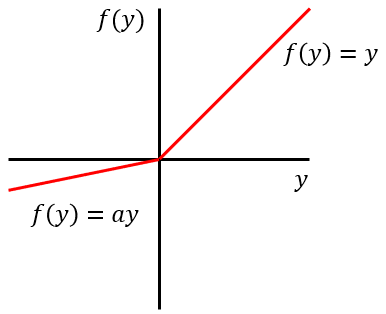
\includegraphics[scale=0.5]{figuren/fig4.png}
    \caption{The Leaky Rectified Linear unit function. Where by default $a=0.2$.}
    \label{fig:leakyrelu}
\end{figure}

A schematic representation of the training process is visualised in Figure \ref{fig:gantraining} . While playing this minimax game, the discriminator tries to tell whether the generators output belongs to the real data distribution or not. The generators tries to outsmart the discriminator, indirectly learning to generate artificial data which corresponds to the real data distribution. More formally, the distribution of the output from the generator $p_g$ over the real data $\mathbf{x}$ with distribution $p_{data}$ is learned as follows. During training the generators input is a 100 dimensional latent vector $\boldsymbol{z}$ which is randomly sampled from a Gaussian distribution $p_{\boldsymbol{z}}$ with mean $\mu=0$ and a standard deviation of $\sigma=1$, i.e. $\mathcal{N}(0,1)$. This noisy latent vector describes a random position in the 100 dimensional parameter space of the original data. Note that this presumes the original dataset being able to be encoded in a 100 dimensional latent space. Essentially this is random noise as an input for the generator. The transformation from the latent space to the generated data is described as $G(\boldsymbol{z}|\boldsymbol{\theta_G})$, where $\boldsymbol{\theta_G}$ are the weights from the generator. In other words, $G(\boldsymbol{z})$ is a generated image $\boldsymbol{y}$. The probability that $\boldsymbol{x}$ comes from $p_{data}$ is described as $D(\boldsymbol{x})$. If $D$ is doing a perfect job, the expected outputs would be $D(\boldsymbol{x})=1$ and $D(\boldsymbol{y})=0$. However, once both $D$ and $G$ are converged, $D$ no longer knows whether $D(\boldsymbol{x})$ or $D(\boldsymbol{y})$ belongs to the real data distribution or not. Meaning that in a perfect situation $p_g \cong p_{data}$ and $D(\boldsymbol{x})=$D(\boldsymbol{y})$=\frac{1}{2}$. The loss function for this minimax game is given by Equation \ref{eq:ganloss}, formally known as the GAN loss function \cite{goodfellow2014generative}. As described in chapter \ref{neuralnetworks} , the solution to this function is approximated by using gradient descent.
\begin{equation}
    \min_{G} \max_{D} V(D,G) = \mathbb{E}_{\boldsymbol{x} \sim p_{data}} [\log(D(\boldsymbol{x})] + \mathbb{E}_{\boldsymbol{z} \sim p_{z}} [\log(1-D(G(\boldsymbol{z}))]
    \label{eq:ganloss}
\end{equation}
Where $\mathbb{E}_{\boldsymbol{x} \sim p_{data}}$ and $\mathbb{E}_{\boldsymbol{z} \sim p_{z}}$ are empirical risk functions and $V$ is a value function \cite{goodfellow2014generative}. Essentially Equation \ref{eq:ganloss} describes that the (indirect) generators loss $\mathbb{E}_{\boldsymbol{z} \sim p_{z}} [\log(1-D(G(\boldsymbol{z}))]$ has to be minimized, while the discriminator loss $\mathbb{E}_{\boldsymbol{x} \sim p_{data}} [\log(D(\boldsymbol{x})]$ has to be maximised during training.   

\begin{figure} [!htb]
    \centering
    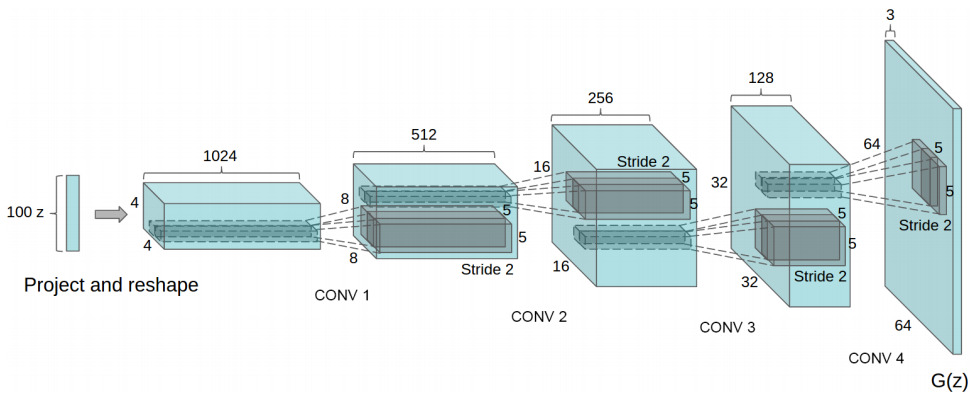
\includegraphics[scale=0.5]{figuren/fig5.png}
    \caption{The original DCGAN generator architecture. The input of the model is a 100 dimensional latent vector. The first convolutional layer consists of 1024 kernels of size 4x4. The second convolution layer consists of 512 kernels of size 8x8, and so on. The final output $G(z)$ is a 64x64x3 image, i.e. a 64x64 colour image in Red Green Blue (RGB).}
    \label{fig:dcganarch}
\end{figure}

The generators architecture of the original DCGAN model is visualized in Figure \ref{fig:dcganarch} . On the left the initial 100 dimensional latent vector is seen, which undergoes 4x4 convolutions by 1024 kernels and eventually the generated image $G(\boldsymbol{z})$ is returned by the network. The discriminator consists of the same architecture, but in reverse with a one dimensional sigmoid output. This sigmoid output has a range from 0 to 1 and is defined by:
\begin{equation}
    f(\boldsymbol{h}_{final}) = \frac{1}{1+e^{-\boldsymbol{h}_{final}}}
    \label{eq:mapping}
\end{equation}
Where $\boldsymbol{h}_{final}$ is the output of the final hidden layer.




\subsection{Wasserstein Generative Adversarial Network with Gradient Penalty}
Currently there are lots of different types of GANs, most of them focusing on solving one single thing, the convergence problems that GANs currently face. One well known problem is vanishing gradient, meaning that the gradient of the discriminator becomes too small and starts to approximate zero. Meaning that the discriminator is no longer learning, forcing the generator to also stop learning. This is where the Wasserstein Generative Adversarial Network with Gradient Penalty (WGAN-GP) comes in \cite{gulrajani2017improved}. 

The WGAN-GP is a new loss function which is supposed to be more stable during training and tackle the problem of vanishing gradient descent. WGAN-GP is the improved version of Wasserstein GAN (WGAN) as described by \cite{arjovsky2017wasserstein}:
\begin{equation}
    \min_{G} \max_{D \in \mathcal{D}} V(D,G) = \mathbb{E}_{\boldsymbol{\tilde{x}} \sim p_g} [D(\boldsymbol{\tilde{x}})] - \mathbb{E}_{\boldsymbol{x} \sim p_{data}} [D(\boldsymbol{x})]
    \label{eq:wgan}
\end{equation}
Where $\mathcal{D}$ is the set of 1-Lipschitz functions and for readability $\boldsymbol{\tilde{x}}=G(\boldsymbol{z})$. WGAN-GP adds a gradient penalty term to the WGAN equation, creating the WGAN-GP loss function \cite{gulrajani2017improved}:

\begin{equation}
    \min_{G} \max_{D \in \mathcal{D}} V(D,G) = \mathbb{E}_{\boldsymbol{\tilde{x}} \sim p_g} [D(\boldsymbol{\tilde{x}})] - \mathbb{E}_{\boldsymbol{x} \sim p_{data}} [D(\boldsymbol{x})] + \lambda \mathbb{E}_{\boldsymbol{\tilde{x}} \sim p_g} [(\mid \mid \nabla_{\tilde{\boldsymbol{x}}} D(\boldsymbol{\tilde{x}}) \mid \mid _2 - 1 )^2]
    \label{eq:wgangploss}
\end{equation}
Where $\lambda$ is a penalty coefficient, a hyperparameter telling how large of an influence the gradient penalty term has on the loss function. The subscript 2 in the last part of the equation represents the L2 norm \cite{ng2004feature}. Whereas ExoGAN is trained by using Equation \ref{eq:ganloss} , SRON-GAN is trained by using Equation \ref{eq:wgangploss} \cite{zingales2018exogan}. This is due to WGAN-GP being more stable during training than the original GAN loss function.

\subsection{Semantic Image Inpainting}\label{semantic image inpainting}

\begin{figure} [!htb]
    \centering
    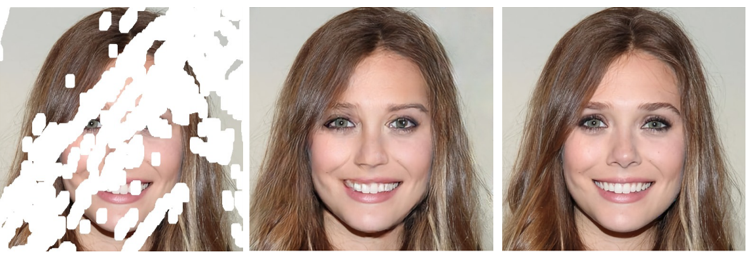
\includegraphics[scale=0.6]{figuren/fig6.png}
    \caption{An example of semantic image inpainting performed by NVIDIA on a 512x512 RGB image \cite{liu2018image}. From left to right: masked input, the inpainted result and the ground truth image. Notice how within the inpainted image the symmetry of the eyes is not in agreement with the ground truth image.}
    \label{fig:inpainting-nvidia}
\end{figure}


Once a DCGAN is converged, one of its' applications is to use it for semantic image inpainting \cite{yeh2017semantic}. In this process the generator and discriminator are used to realistically fill in missing data from a corrupted image, as seen in Figure \ref{fig:inpainting-nvidia} . This is done by solving the following loss function, again by gradient descent \cite{yeh2017semantic}:
\begin{equation}
    \boldsymbol{\hat{z}} = \arg \min_{\boldsymbol{z}} {\mathcal{L}_c(\boldsymbol{z}|\boldsymbol{y},\boldsymbol{M}) + \mathcal{L}_p (\boldsymbol{z})}
    \label{eq:inpaintingloss}
\end{equation}
Where $\mathcal{L}_c(\boldsymbol{z}|\boldsymbol{y},\boldsymbol{M})$ is the contextual loss, $\mathcal{L}_p (\boldsymbol{z})$ the perceptual loss, $\boldsymbol{z}$ a latent vector, $\boldsymbol{y}$ the corrupted image and $\boldsymbol{M}$ a mask. The mask has the same shape as $\boldsymbol{y}$ and in the simplest case it is a binary mask, having the value of 0 at places where pixels are missing and values of 1 at places where pixels are not missing from $\boldsymbol{y}$. The goal of Equation \ref{eq:inpaintingloss} is to find a $\boldsymbol{z}$ which properly fits the context of $\boldsymbol{y}$ and also is a realistic fit according to the discriminator. Once done successfully, the best latent vector $\boldsymbol{\hat{z}}$ has been found. The contextual loss is defined as \cite{yeh2017semantic}:
\begin{equation}
    \mathcal{L}_c(\boldsymbol{z}|\boldsymbol{y},\boldsymbol{M}) = ||\boldsymbol{M} \odot (G(\boldsymbol{z})-\boldsymbol{y})||_1
    \label{eq:contextual_loss}
\end{equation}
Where $\odot$ is the Hadamard product \cite{horn1990hadamard}, denoting element wise multiplication of the matrices and the subscript $1$ denotes the L1 norm \cite{ng2004feature}. Conceptually Equation \ref{eq:contextual_loss} tries to minimise the error between the known pixels of the inpainted image, and the known pixels of the original image. Meaning that it will try to find a $\boldsymbol{z}$ which lets $G$ return the same image as the original image $\boldsymbol{y}$, for the known pixels. The perceptual loss is defined as \cite{yeh2017semantic}:
\begin{equation}
    \mathcal{L}_p (\boldsymbol{z}) = \lambda \log(1-D(G(\boldsymbol{z}))
\end{equation}
Where $\lambda$ is a hyperparameter to keep the preferred balance between the contextual and perceptual loss. Notice how $D$ and $G$ are only used as functions. During the inpainting process, the initially randomly chosen latent vector $\boldsymbol{z}$ is adjusted with gradient descent to minimise Equation \ref{eq:inpaintingloss} . Once converged, the best latent vector $\boldsymbol{\hat{z}}$ has been found, where $\boldsymbol{\hat{z}}  \subseteq \boldsymbol{z}$. After which the inpainted image $\boldsymbol{\hat{x}}$ is retrieved through \cite{yeh2017semantic}:
\begin{equation}
    \boldsymbol{\hat{x}} = G(\boldsymbol{\hat{z}}) \odot (1-\boldsymbol{M})+\boldsymbol{M}\odot \boldsymbol{y}
\end{equation}







\subsection{Loss Functions} \label{lossfunctions_subchapter}
Within this subchapter the previously presented loss functions are simplified. The goal of this simplification is to get rid of the mathematical formalisms used and present functions which are relatively easy to implement in for example Python.

Take the GAN loss function, Equation \ref{eq:ganloss}. The first step is to get rid of all rigorous notations and use a more general notation. The value function $V$ can be exchanged for a more recognised function symbol $f$. The empirical loss function $\mathbb{E}$ can be completely left out. Which changes
\begin{equation}
    \min_{G} \max_{D} V(D,G) = \mathbb{E}_{\boldsymbol{x} \sim p_{data}} [\log(D(\boldsymbol{x})] + \mathbb{E}_{\boldsymbol{z} \sim p_{z}} [\log(1-D(G(\boldsymbol{z}))]
    \tag{\ref{eq:ganloss}}
\end{equation}

to 

\begin{equation}
    \min_{G} \max_{D} f(D,G) = \log(D(\boldsymbol{x})) + \log(1-D(G(\boldsymbol{z}))
    \label{eq:ganloss_simplified}
\end{equation}

Note that the expressions of the real data $\boldsymbol{x}$ coming from the real data distribution $\mathbb{p_{data}}$ is lost. Just like $\boldsymbol{z} \sim p_{z}$ is lost. This does not have any practical consequences. Equation \ref{eq:ganloss_simplified} is the simplified GAN loss function. Where $\min_{G}$ denotes that $G$ has to be minimised and $\max_{D}$ denotes that $D$ has to be maximised. As a reminder, $D$ has a sigmoid function at its output. The sigmoid function has a range of 0 to 1.

This minimisation and maximisation problem is the so called two player minimax game. To clarify this further, this minimax game is broken down into two stages. One with the goal of the discriminator and one with the goal of the generator. The first stage consists of the goal to maximise the capability of $D$ to discriminate between real and fake, this is the $\max_{D}$ part. The second stage consists of $G$ learning to fool $D$, this is the $\min_{G}$ part. For the first stage, a perfect discriminator, the outputs would be as follows:
    
    
\begin{equation}
    D(\boldsymbol{x}) = 1
    \nonumber
\end{equation}
\begin{equation}
    D(G(\boldsymbol{z})) = 0
    \nonumber
\end{equation}
Whereas in the second stage, a perfect generator, the output would be:
\begin{equation}
    D(G(\boldsymbol{z})) = 1
    \nonumber
\end{equation}
Since both models are competing with each other, ideally $D$ is no longer able to discriminate between real and fake. Which translates to the generator no longer being able to improve. Meaning that the output of the discriminator would become:
\begin{equation}
    D(\boldsymbol{x}) = D(G(\boldsymbol{z})) = 0.5
    \nonumber
\end{equation}
The same simplification can be applied to the WGAN and WGAN-GP loss functions. This changes the WGAN loss function from 
\begin{equation}
    \min_{G} \max_{D \in \mathcal{D}} V(D,G) = \mathbb{E}_{\boldsymbol{\tilde{x}} \sim p_g} [D(\boldsymbol{\tilde{x}})] - \mathbb{E}_{\boldsymbol{x} \sim p_{data}} [D(\boldsymbol{x})]
    \tag{\ref{eq:wgan}}
\end{equation}
to 
\begin{equation}
    \min_{G} \max_{D \in \mathcal{D}} f(D,G) = D(G(\boldsymbol{z})) - D(\boldsymbol{x}).
    \label{eq:wgan_simplified}
\end{equation}
Where $\boldsymbol{\tilde{x}}$ has been substituted back for $G(\boldsymbol{z})$. This loss function translates to the same goal, in a different mathematical formulation. Both Equation \ref{eq:ganloss_simplified} and \ref{eq:wgan_simplified} have one problem, they are sensitive to vanishing gradient. Meaning that the gradient of the weights often can start to approximate zero, which in returns stops the models from learning any further. To combat this, a gradient penalty term is added to the WGAN loss function \cite{gulrajani2017improved}. This creates the WGAN-GP loss function \cite{arjovsky2017wasserstein}: 
\begin{equation}
    \min_{G} \max_{D \in \mathcal{D}} V(D,G) = \mathbb{E}_{\boldsymbol{\tilde{x}} \sim p_g} [D(\boldsymbol{\tilde{x}})] - \mathbb{E}_{\boldsymbol{x} \sim p_{data}} [D(\boldsymbol{x})] + \lambda \mathbb{E}_{\boldsymbol{\tilde{x}} \sim p_g} [(\mid \mid \nabla_{\tilde{\boldsymbol{x}}} D(\boldsymbol{\tilde{x}}) \mid \mid _2 - 1 )^2]
    \tag{\ref{eq:wgangploss}}
\end{equation}
Which when simplified becomes:
\begin{equation}
    \min_{G} \max_{D \in \mathcal{D}} f(D,G) = D(G(\boldsymbol{z})) - D(\boldsymbol{x}) + (\mid \mid \nabla_{G(\boldsymbol{z})} D({G(\boldsymbol{z})}) \mid \mid _2 - 1 )^2
\end{equation}









\subsection{Latest Developments}
GANs have the ability to learn the latent space of a data distribution. Their generative ability is something previously unseen for regular neural networks and this makes them especially powerfull. GANs are starting to get applied to e.g. dark energy, radio interferometry, fluid dynamics, chaotic dynamical systems and radiotherapy \cite{li2019model,glaser2019radiogan,werhahn2019multi,wu2019enforcing,kazemifar2019mri}. They are also actively used at CERN in the search for new physics, data modelling and analysis \cite{lin2019machine, di2019dijetgan, hashemi2019lhc, chekalina2018generative, paganini2018calogan, maevskiy2019fast, paganini2019machine}. 


However, GANs do have some rough edges to them. This is something which is often not discussed within the work where they are used. GANs are currently an active research area and new developments to their performance are constantly being made. Apart from the downsides of requiring immense datasets, computational power and computational time to train, there are more drawbacks than this. Neural networks in general are sensitive to their hyperparameters. GANs surpass this sensitivity significantly. To put this in perspective; When for example the learning rate is changed by 0.01 for a regular neural neural network, an accuracy change of 2\% might take place. Do this with a GAN and it might completely fail to converge, although it previously was doing fine in training. Previously mentioned pitfalls are merely a difficulty in the user friendliness of GANs, compared to other problems they come with. Some well known and hard to solve, or currently unsolved problems are (mode) collapse, GAN artifacts, model validation and the inability to converge depending on the loss function or dataset used. 

When mode collapse takes place the generator learns to produce one solution, always fooling the discriminator. The term collapse is described as follows. The generator and discriminator are out of balance during training. An example would be where the discriminator is stronger than the generator during training. In this case the generator fails to keep up with the rate at which the discriminator is learning. This eventually leads to a collapse of the generator, where it starts to output e.g. purely noise or fully black and white images. The same thing can happen to the discriminator. This problem is usually dealt with by e.g. training the generator two times per batch, where the discriminator is only trained once. Both mode collapse and collapse do not need to happen at the start of training. It might aswell occur hours or days into training, despite the model seeming to converge properly before this event. Due to this reason the training process has to be constantly monitored.

GAN artifacts are artifacts visible in the generated images. If the GAN is supposed to produce faces, examples of artifacts could be unrealistic representations of the persons hair, eyes and symmetry within the face. Take for example Figure \ref{fig:inpainting-nvidia}, the symmetry of the face appears to be unrealistic. Currently the state of the art GANs still contain these artifacts. Another form of artifacts are checkerboard patterns as seen in Figure \ref{fig:checkerboard}. These are patterns of lighter and darker pixels, occurring due to the way the convolution kernels are aligned withing the generator \cite{odena2016deconvolution}. One solution to this would be letting the model train for longer. While another solution would be to rearrange the kernels used, use different convolution algorithms, or a combination of both. The latter sounds easy, but is a difficult and time consuming task.

\begin{figure} [!htb]
    \centering
    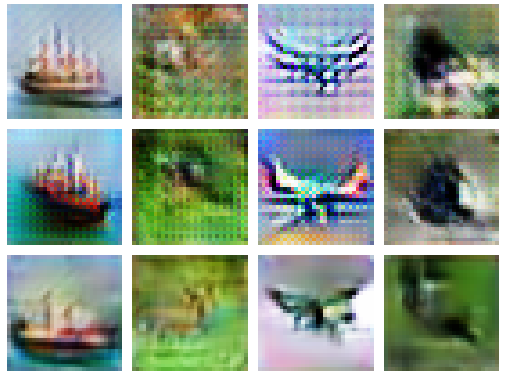
\includegraphics[scale=0.6]{figuren/checkerboard.png}
    \caption{Checkerboard patterns occurring in generated images. Going down from the top row, the network architecture is changed to minimise the visibility of the checkerboard pattern. Image source: \cite{odena2016deconvolution}.}
    \label{fig:checkerboard}
\end{figure}


















\subsection{Previous Work: ExoGAN} \label{exogan}
In this subsection ExoGAN \cite{zingales2018exogan}, its theory, methods and result are discussed. This is done because SRON-GAN is completely inspired by the work done by \cite{zingales2018exogan}. ExoGAN is a DCGAN designed for $33\times33$ black and white images. ExoGAN uses Equation \ref{eq:ganloss} as the loss function. Both the discriminator and generator architecture of ExoGAN are found in Table \ref{table:exogan_network_architecture}. Notice how the network architecture is different from the DCGAN in Figure \ref{fig:dcganarch}. ExoGAN uses different kernel sizes for the filters, hence their fourth layer has a size of 33x33 instead of 32x32. Finally the hyperparameters are found in Table \ref{table:exogan_hyperparams}.

\begin{figure} [!htb]
    \centering
    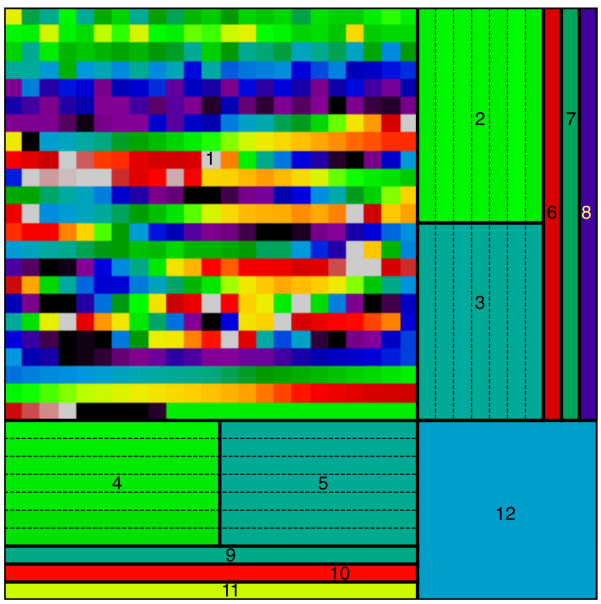
\includegraphics[scale=0.35]{figuren/exogan_aspa.png}
    \caption{An example of a false-colour ASPA from the ExoGAN dataset \cite{zingales2018exogan}. Where area 1 encodes the spectrum, area 2-5 the local minimum and maximum values used for the spectrum normalisation, area 6-11 the atmospheric model features and area 12 encodes the $\mathrm{H2_0}$ abundance.}
    \label{fig:exogan_aspa}
\end{figure}


The ExoGAN dataset consists of $10^7$ forward models generated by the TauREx retrieval code \cite{waldmann2015tau, waldmann2015rex}. The forward model parameters are sampled in 10 bins within the parameter ranges as given in Table \ref{table:exogandatasetparameters}. The dataset is split into 90\% training and 10\% testing. One important detail which the authors did not mention is for how many iterations ExoGAN has been trained. All other training details are in agreement with previous (DC)GAN literature. One key aspect of ExoGAN is the way the input images are designed, see Figure \ref{fig:exogan_aspa}. Each input image consists of a so called Atmospheric Spectrum and Parameter Array (ASPA). An ASPA encodes the transmission spectrum and its corresponding parameters and features into an image. ASPA creation is discussed in Chapter \ref{ASPA encoding and decoding}. Note that Figure \ref{fig:exogan_aspa} is a false-colour representation of the originally black and white ASPA. Area 1 encodes the spectrum between 1$\mu$m and 50$\mu$m, which is normalised in 14 bins to maximally amplify the $\mathrm{H_2O}$ signature inside the spectrum. Area 2 to 5 encode the normalisation factors used to normalise the spectrum bins. Area 6 to 12 encode the atmospheric trace-gas volume mixing ratio's, planet mass, planet radius and planet temperature as previously seen in Table \ref{table:exogandatasetparameters} \cite{zingales2018exogan}.

\begin{figure} [!htb]
    \centering
    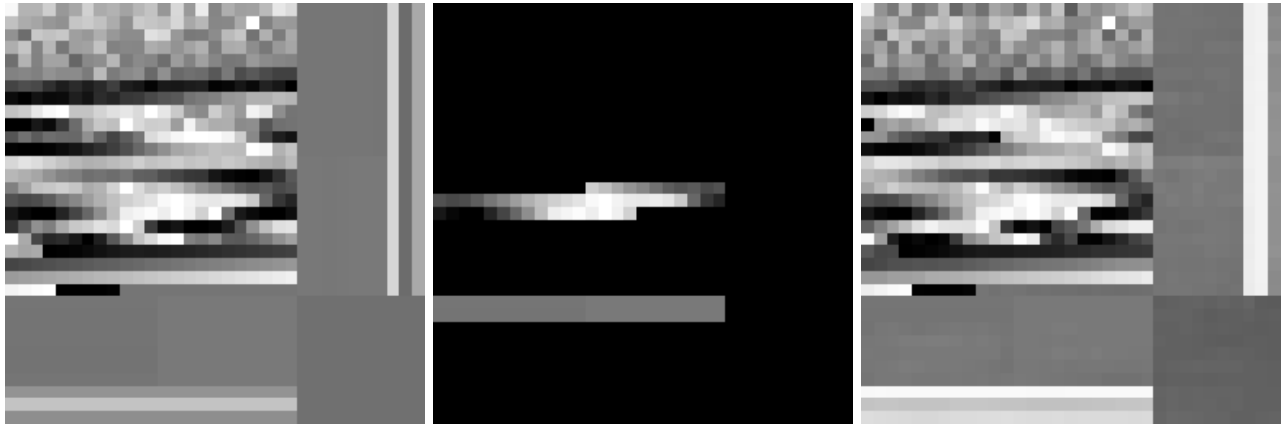
\includegraphics[scale=0.3]{figuren/exogan_mask_inpainting.png}
    \caption{On the left the ground-truth ASPA. In the middle is the masked ASPA, in this case only the wavelengths from Hubble Space Telescope's Wide Field Camera 3 (WFC3) are left as known values. On the right is the inpainted ASPA \cite{zingales2018exogan}.}
    \label{fig:exogan_aspa_inpainting}
\end{figure}


Once trained, an accuracy test is performed on 1000 ASPAs from the test dataset. Summarised, per ASPA, 1000 noisy instances of the observed spectrum are created. Where each of these instances has a random mask consisting of missing parameters, missing spectral ranges or both. An example of such a mask is shown in Figure \ref{fig:exogan_aspa_inpainting}. Semantic image inpainting is performed as described in Chapter \ref{semantic image inpainting} and the accuracy per retrieved parameter $A$ is calculated by \cite{zingales2018exogan}:

\begin{equation}
    A(\phi ,\sigma_\phi) = \frac{1}{N} \sum_{i}^{N} \frac{(\phi_{i,recon}-\phi_i)^2}{\phi_i^2+\sigma_{\phi_i}^2}
\end{equation}

Where $N$ is the number of inpainted ASPA instances, $\phi$ is the ground-truth parameter value, $\phi_{recon}$ the retrieved parameter value and $\sigma_\phi$ its corresponding error. The results of ExoGAN are shown in Table \ref{table:exogantestresults} . It is worth nothing that it is unclear how $\sigma_{\phi}$ has been defined.



















%%%%%%%%%%%%%%%%%%%%%%%%%%%%%%%%%%%%%%%%%%%%%%%%%%%%%%%%%%%%%%%%%%%%%%%%%%%%%%%%%%
